\documentclass[acmsmall,screen]{acmart}
\usepackage{colortbl}
\usepackage{amsmath}
\usepackage{xcolor}
\usepackage{tikz}
\usepackage{pgfplots}
\pgfplotsset{compat=1.18}
\usetikzlibrary{shapes.geometric,arrows.meta,positioning,
  fit,calc,decorations.pathreplacing,backgrounds,patterns,shadows}

\newcommand{\nCanonicalAgentic}{827}

\newcommand{\traceLinEpGJ}{254.5}

\newcommand{\EpG}{\textsc{EpG}}

\newcommand{\traceAttemptOneJ}{2256.1}

\newcommand{\traceAttemptTwoJ}{1358.4}

\newcommand{\traceEpGJ}{3614.5}

\newcommand{\traceOOI}{14.2}

\newcommand{\meanEpGLinClean}{205.3}

\newcommand{\meanEpGAgClean}{888.1}

\newcommand{\headlineOOIClean}{4.33}

\begin{document}

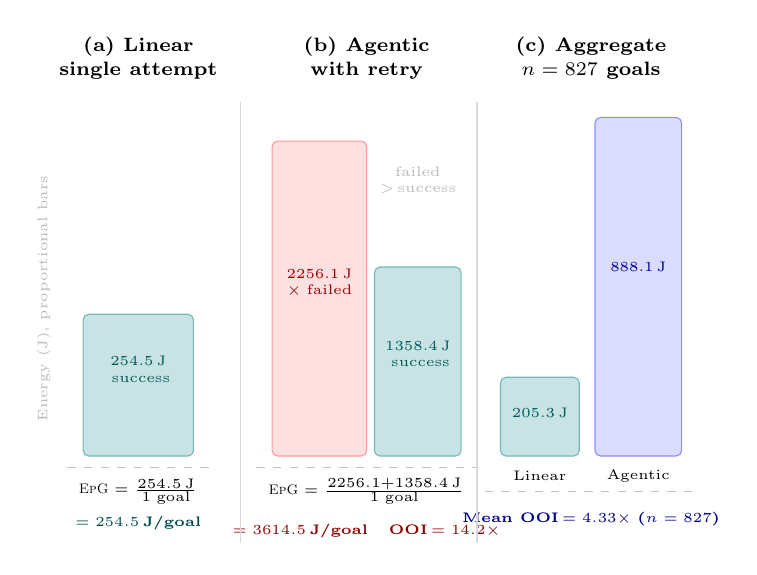
\begin{tikzpicture}[
  >=Stealth,
  font=\scriptsize,
  bar/.style={rounded corners=2pt, line width=0.4pt},
  ok/.style={bar, fill=teal!22, draw=teal!55},
  fail/.style={bar, fill=red!12, draw=red!40},
  agg/.style={bar, fill=blue!14, draw=blue!45},
  lbl/.style={font=\tiny, align=center},
  hdr/.style={font=\scriptsize\bfseries, align=center},
  dim/.style={gray!50, line width=0.3pt, dashed},
  node distance=0.0cm,
]
 
%% ── Scale: 3614.5J = 52mm ────────────────────────────────
%% Panel A: linear 254.5J = 254.5/3614.5*52mm = 3.66mm ≈ too small
%% Use per-panel scale for clarity:
%% Panel A: 254.5J -> 18mm (single bar, own scale)
%% Panel B: attempt1=2256.1J->40mm, attempt2=1358.4J->24mm (same scale, total=64mm)
%% Panel C: linear=205.3J->10mm, agentic=888.1J->43mm (same scale)
 
%% ── Panel labels ──────────────────────────────────────────
\node[hdr] at (1.1,  5.2) {(a) Linear};
\node[hdr] at (1.1,  4.9) {single attempt};
\node[hdr] at (4.0,  5.2) {(b) Agentic};
\node[hdr] at (4.0,  4.9) {with retry};
\node[hdr] at (6.85, 5.2) {(c) Aggregate};
\node[hdr] at (6.85, 4.9) {$n=\nCanonicalAgentic{}$ goals};
 
%% ── PANEL A: Linear 254.5J ────────────────────────────────
\fill[ok] (0.4, 0) rectangle (1.8, 1.8);
\node[lbl, text=teal!70!black] at (1.1, 1.1)
  {\traceLinEpGJ\,J\\\checkmark\;success};
 
%% denominator brace
\draw[dim] (0.2, -0.15) -- (2.0, -0.15);
\node[lbl] at (1.1, -0.45)
  {$\EpG = \frac{\traceLinEpGJ\,\mathrm{J}}{1\;\mathrm{goal}}$};
\node[font=\tiny\bfseries, text=teal!60!black] at (1.1, -0.85)
  {$=\traceLinEpGJ$\,J/goal};
 
%% ── PANEL B: Agentic attempt1 (failed) + attempt2 (success) ──
%% attempt1: 2256.1J -> 40mm = 4.0cm
%% attempt2: 1358.4J -> 24mm = 2.4cm
%% bars side by side with gap
 
\fill[fail] (2.8, 0) rectangle (4.0, 4.0);
\node[lbl, text=red!60!black] at (3.4, 2.2)
  {\traceAttemptOneJ\,J\\$\times$\;failed};
 
\fill[ok]   (4.1, 0) rectangle (5.2, 2.4);
\node[lbl, text=teal!70!black] at (4.65, 1.3)
  {\traceAttemptTwoJ\,J\\\checkmark\;success};
 
%% sum brace
\draw[dim] (2.6, -0.15) -- (5.4, -0.15);
\node[lbl] at (4.0, -0.45)
  {$\EpG = \frac{\traceAttemptOneJ+\traceAttemptTwoJ\,\mathrm{J}}
                {1\;\mathrm{goal}}$};
\node[font=\tiny\bfseries, text=red!55!black] at (4.0, -0.95)
  {$=\traceEpGJ$\,J/goal\quad OOI\,$=\traceOOI\times$};
 
%% annotation: failed > success
\node[font=\tiny, gray!55, align=center] at (4.65, 3.5)
  {failed\\$>$\,success};
 
%% ── PANEL C: Aggregate means ──────────────────────────────
%% linear 205.3J -> 205.3/888.1*43mm = 9.95mm ≈ 1.0cm
%% agentic 888.1J -> 43mm = 4.3cm
 
\fill[ok]  (5.7, 0) rectangle (6.7, 1.0);
\node[lbl, text=teal!70!black] at (6.2, 0.55)
  {\meanEpGLinClean\,J};
 
\fill[agg] (6.9, 0) rectangle (8.0, 4.3);
\node[lbl, text=blue!60!black] at (7.45, 2.4)
  {\meanEpGAgClean\,J};
 
%% axis labels
\node[font=\tiny, align=center] at (6.2, -0.25) {Linear};
\node[font=\tiny, align=center] at (7.45, -0.25) {Agentic};
 
\draw[dim] (5.5, -0.45) -- (8.2, -0.45);
\node[font=\tiny\bfseries, text=blue!55!black] at (6.85, -0.80)
  {Mean OOI\,$=\headlineOOIClean\times$\;($n=\nCanonicalAgentic{}$)};
 
%% ── Panel dividers ────────────────────────────────────────
\draw[gray!30, line width=0.5pt]
  (2.4, -1.1) -- (2.4, 4.5);
\draw[gray!30, line width=0.5pt]
  (5.4, -1.1) -- (5.4, 4.5);
 
%% ── Y-axis label ──────────────────────────────────────────
\node[rotate=90, font=\tiny, gray!55] at (-0.1, 2.0)
  {Energy (J), proportional bars};
 
\end{tikzpicture}

\end{document}